%
\section{Biometric Key Generation \\from HMOG features}
\label{sec:bkg}

%
\begin{table*}[t]
\caption{List of symbols used in this section.}
\begin{tabular}{|l|l||l|l|}
\hline
$C$ 							& Error-correcting code (vector space over $\Z_p$). & $\delta = (x-c)$					& Discretize biometric sample $x$ masked by $c$. \\

%
$n$ 							& Number of biometric features, as well as length of $C$. & $\gamma$					& Fuzzy commitment \\
$p$ 							& Alphabet size of $C$. ($p$ is a prime number larger $n$.)  & ${\sf d\_range}_{{F}_i}$			& Upper bound of the range of ${\sf DS}_{{F}_i}$ \\
%
$l$							& Dimension of $C$ (size of the basis of $C$).  & ${\sf min}_{{F}_i}, {\sf max}_{{F}_i}$ & Minimum and maximum values of $F_i$	 \\ 
$w_L(\cdot), d_L(\cdot,\cdot)$			& Lee weight and Lee distance functions. & $\sigma_i$				& Standard deviation of $F_i$ \\
%
$z$							& System-wide public constant or user PIN/password. & $x_i$  		& Instance of $F_i$ \\ 
%
$c = (c_1, \ldots, c_n)$			& Codeword from $C$. & ${F}_i$		& Biometric feature $i$\\
$x = (x_1, \ldots, x_n)$			& Discretized biometric sample. & & \\




%


%


\hline
\end{tabular}
\label{tbl:bkg-symbols}
\end{table*}
%

In this section, we evaluate the performance of HMOG features for biometric key 
generation (BKG). For this purpose, we introduce our BKG construction, which 
extends and generalizes the fuzzy commitment scheme of Juels et 
al.~\cite{fuzzy_commitment}. While the technique in~\cite{fuzzy_commitment} operates on features represented using a single bit, our BKG construction represents features as symbols of an alphabet of arbitrary prime size $p$. Our BKG relies on Reed-Solomon error correcting codes~\cite{rot06} in Lee metric~\cite{lee58}. Notation used in this section is presented in Table~\ref{tbl:bkg-symbols}.


\paragraph{Preliminaries}
BKG uses  biometric information to prevent unauthorized access to cryptographic keys; these keys can then be used, e.g., to encrypt/decrypt sensitive information. The process of protecting a key is referred to as {\em 
committing}, and the outcome of this process is a {\em commitment}. Given a 
commitment, the cryptographic key is reconstructed by {\em decommiting} (or {\em 
opening}) it, using information from a biometric signal. 
Informally, a BKG construction is secure if a key committed using a biometric signal $s$ can be opened only using a signal $s'\approx s$, and both $s$ and $s'$ are from the same user. 

BKG techniques use error-correcting codes to address natural variations among 
different biometric samples from the same users.  An error-correcting code is 
defined as a set $C$ of codewords. Typically, there are two functions associated 
with a code: ${\sf encode(\cdot)}$ and ${\sf decode(\cdot)}$. The former maps a 
message to a codeword; the latter---a possibly perturbed codeword to the original 
codeword. 
The ${\sf decode(\cdot)}$ function is designed to maximize the probability of 
correct decoding. 

\subsection{Our Construction}
\paragraph{Scaling and Discretization}
BKG techniques work on discrete values, instead of real values. Therefore, the 
user first performs scaling and discretization of the feature vector representing 
her biometric.
Each feature $F_i$ is assigned a discretization range $[0, {\sf d\_range}_{F_i}]$, where ${\sf d\_range}_{F_i} \in \{(p-1)/2,\ldots, p-1\}$ is negatively correlated to the standard deviation $\sigma_i$ of $F_i$ (i.e., if $\sigma_i < \sigma_j$, then ${\sf d\_range}_{F_i} > {\sf d\_range}_{F_j}$).

Let $x_{i}$ be an instance of ${F_i}$, and ${\sf min}_{F_i}$ and ${\sf max}_{F_i}$ be respectively the typical minimum and maximum value of ${F_i}$. Discretization and scaling are performed as:
%
\[\small
{\sf DS}_{{{F_i}}}(x_i) = 
\resizebox{0.8\linewidth}{!}{$
\begin{cases}
0 & x_i<{\sf min}_{F_i} \\ \\
\left\lfloor {\sf d\_range}_{F_i}\cdot\left(\frac{ x_i-{\sf min}_{F_i}}{{\sf max}_{F_i}-{\sf min}_{F_i}}\right)\right\rfloor & {\sf min}_{F_i} \leq x_i \leq {\sf max}_{F_i} \\ \\
{\sf d\_range}_{F_i} & x_i>{\sf max}_{F_i} \\
\end{cases}$}
\]
%


\paragraph{Committing a Key}
To commit a cryptographic key using $n$ biometric features, the user 
selects a random codeword $c$ of length $n$ from $C\subset(\Z_p)^n$. The key is 
computed as $k = \PRF_c(z|0)$, where $\PRF$ is a pseudorandom function family, 
$z$ is a system-wide public constant and ``$|$'' denotes string concatenation. (BKG can be augmented with a second authentication factor by setting $z$ to a user-provided password.) $c$ is then committed using the user's biometrics as discussed next. 
Let $x = (x_1, \ldots, x_n)$ be a scaled and discretized feature vector. The user 
computes $\delta = (x-c) = (x_1-c_1, \ldots, x_n-c_n)$ and publishes commitment $
\gamma = (\PRF_c(z|1), \delta)$.

The user computes $k$ from $\gamma$ and her biometric signals (and possibly a 
password $z$) as follows. She extracts biometric features from the signal, and 
encodes them as $y=(y_1,\ldots,y_n)$. Then, she computes $c' = {\sf decode}(y-
\delta)$. If $\PRF_{c'}(z|1) = \PRF_c(z|1)$, then $k=\PRF_{c'}(z|0)$ with overwhelming probability. 

Asymptotic complexity of BKG key retrieval is dominated by one instance of Euclidean algorithm and one matrix-vector multiplication, both in $O(n^2)$ finite field operations in a field of size $p \geq n$. Security of our construction is analyzed in Appendix~\ref{sec:security}.  %

\paragraph{Using Lee-metric Decoding for BKG}
Distance between feature vectors is defined using the Lee distance~\cite{lee58}---a discrete approximation of SM:

\begin{definition}[Lee weight]
Let $p$ be an odd prime. The \emph{Lee weight} of element $x \in \Z_p$ is defined as $w_L(x) = \min|x'|$, for $x' \equiv x \bmod{p}$. %
The \emph{Lee weight} of vector $x = (x_1,\ldots, x_n) \in (\Z_p)^n$ is defined as the sum of Lee weights of its elements, i.e., $w_L(x) = \sum_{i=1}^n{w_L(x_i)}$.
\end{definition}

\begin{definition}[Lee distance]
The \emph{Lee distance} of vectors $x, y \in \Z_p$ is the Lee weight of their difference, i.e., $d_L(x, y) = w_L(x - y)$. 
\end{definition}
In $\Z_2$, the Lee weight coincides with Hamming weight.

%


%
%
We used normalized generalized Reed-Solomon codes from \cite{rot06}, presented next, to implement the ${\sf encode}(\cdot)$ and ${\sf decode}(\cdot)$ functions.
%


%
%
%

\begin{definition}
Let $l \leq n$ and $n\leq p$. A linear $[n, l]$-code over $\Z_p$ is a $l$-dimensional vector subspace of $(\Z_p)^n$. 
 A normalized Reed-Solomon $[n, l]$-code over $\Z_p$ is a linear $[n, l]$-code over $\Z_p$ with parity-check matrix: 
\[ \resizebox{0.55\linewidth}{!}{$
 H = \left( 
 \begin{array}{cccc}
1 & 1   & \ldots & 1 \\
1 & 2   & \ldots & n \\
1 & 2^2 & \ldots & n^2 \\
\multicolumn{4}{c}{\vdots}   \\
1 & 2^{n-l-1} & \ldots & n^{n-l-1} \\
 \end{array} 
 \right)$}
\]
%
and generator matrix:
%
\[ \resizebox{0.55\linewidth}{!}{$
 G = \left( 
 \begin{array}{cccc}
v_1 &     v_2 & \ldots &     v_n \\
v_1 & 2   v_2 & \ldots & n   v_n \\
v_1 & 2^2 v_2 & \ldots & n^2 v_n \\
\multicolumn{4}{c}{\vdots}   \\
v_1 & 2^{l-1} v_2 & \ldots & n^{l-1} v_n \\
 \end{array} 
 \right) $}
\]
\end{definition}

The rows of $G$ form a basis of the nullspace of $H^T$. 

%
%
%
%
To obtain a random codeword from $C$, we select a $l$-tuple $m = (m_1, \ldots, m_l) \in (\Z_p)^l$ uniformly at random, and encode $m$ as $c = mG$. 
%
The Lee distance of $C$ is $2(n-l)$, so for any error $e = (e_1, \ldots, e_n)$ with $w_L(e) < n-l$, ${\sf decode}(c+e) = c$.

%

%
%
%
%
%
%
%

%





%
%
%
%

%

%
%
%
%
%
%
%
%
%
%
%
%

\subsection{Evaluation of HMOG Features on BKG}

To evaluate HMOG features for BKG, we determined their authentication 
accuracy and security against population attacks. We then compared our results with HMOG features to that of tap, key hold, and swipe features under the same metrics.
%

\paragraph{Biometric Accuracy}
Figures~\ref{fig:bkg_sitting} and~\ref{fig:bkg_walking} summarize the results of 
our experiments, performed on our 100-user dataset. We evaluated BKG using the 
features that performed best for authentication. We used 17 and 13 HMOG features in sitting and walking conditions, respectively (see Figure~\ref{fig:fisherFeatures}).


We ran experiments on four different feature subsets: (1)~HMOG-only features; 
(2) 11 tap-only features; (3) 12 (sitting) and 8 (walking) key hold-only features; 
and (4) HMOG and 3 best-performing tap features. For both walking and sitting experiments, feature 
subset (4) provided the best results, i.e., 15\% and 20\% EER respectively, for both one-minute and two-minute scan lengths. For sitting 
experiment, key generation was not possible with (3), as the within-user 
variability of the biometrics signals was too high. 

Sedenka et al.\cite{sedenka2014} showed that Linear Discriminant Analysis (LDA)~\cite{lda} 
improves BKG accuracy on desktop keystroke dynamics. However, HMOG, tap, and 
key hold features on a virtual keyboard did not benefit from LDA. Therefore we do 
not report BKG results with LDA for these features.


\paragraph{Security Against Population Attacks}
EER computed via zero-effort attacks provides limited information on the security 
of a BKG scheme, because it does not take into account all the information 
readily available to the adversary. In particular, with BKG the adversary has 
access to: (1) the commitment~$\gamma$; and (2) an approximation of the 
distribution of the user's biometric signals obtained from  {\em population 
data}. 

Access to $\gamma$ allows the adversary to test whether a particular feature 
vector decommits the key. The adversary can perform this test {\em offline}, 
i.e., with no restrictions on the number of attempts performed (within the limits of the available resources). Therefore, the hardness of ``guessing'' a user's feature vector given 
$\gamma$ is an upper bound on the security of a BKG scheme. 

The adversary can use (2) to guess the user's feature vector more efficiently, 
under the assumption that biometric signals from different users are not 
completely independent. To this end, Ballard et al.~\cite{bal08} proposed the notion 
of \emph{guessing distance}. It is defined as the logarithm of the number of 
guesses necessary to open a 
commitment using feature vectors from multiple impostors.

We instantiated guessing distance in our setting as follows. First, we built a 
commitment $\gamma_i=(\PRF_{c_i}(z|1), \delta_i)$ from the feature vector 
of each user $i$. Then, we used the biometric sample from user $j$ to open all $
\gamma_i$ such that $i\neq j$, and ranked users according to how many 
commitments they were able to open.  Finally, for each user $i$ we select users 
$j\neq i$ following to this ranking, and determined how many attempts were 
required to open $\gamma_i$. Guessing distance was computed as the binary 
logarithm of this value.
%
There might be users $i$ for which no feature vector from other users could open 
$\gamma_i$. We refer to the commitments of these users as {\em non-guessed}.

Table~\ref{tbl:bkg_guessing} summarizes the results of our experiments for one 
minute scans. The lowest EER was achieved by combining HMOG features 
with the tap features selected by mRMR. Overall, HMOG outperformed tap 
features for biometric key generation. Nevertheless, our results show that most 
commitments can be guessed using population data. 

\paragraph{Comparison of HMOG and Swipe Features}
Because there is no previous work on BKG using touch-, accelerometer-, or gyroscope-based features, we compared BKG on HMOG with BKG on touch features extracted from swipes ({\em swipe features} hereafter). For this purpose, we computed swipe features from the datasets of Serwadda et al.~\cite{serwadda2013}. As in \cite{serwadda2013}, we used the whole first session for computing commitments and ten swipes from the second session to perform impostor/genuine {\em open} attempts. 
%
Results are reported in Table \ref{tbl:bkg_guessing}. 

We also performed experiments on the touch dataset of Frank et al.~\cite{frank2013}. However, a large majority of the users could not reliably decommit their own keys. This was due to the large variance between the vectors used to build the commitment, and the one used to open it. Therefore, we did not include these results in this paper.

%




\begin{table*}[ht!]
\centering
\caption{Security of BKG based on HMOG, tap, key hold, and swipe features. %
}
\label{tbl:bkg_guessing}

\begin{tabular}{llllll}
Dataset                              & Features                                                                    & EER    &  \parbox{1.5cm}{Average guessing distance} & \parbox{2cm}{Non-guessed commitments} & $\log_2(|C|)$ \\ \hline
\multirow{3}{*}{Our dataset-sitting} & HMOG                                                                           & 23.4\% & 2.8         & 2\%                    & 19                  \\
%
                                     & HMOG with best 3 tap                                                         & 20.1\% & 2.7         & 1\%                    & 18                  \\
                                     & Tap                                                                          & 25.7\% & 1.6         & 2\%                     & 25                  \\ \hline
\multirow{4}{*}{Our dataset-walking} & HMOG                                                                           & 17.4\% & 2.9         & 2\%                    & 27                  \\
                                     & HMOG with best 3 tap                                                         & 15.1\% &3.2        & 5\%                    & 33                  \\
%
                                     & Tap                                                                          & 28.4\% & 1.9         & 0\%                     & 30                  \\
                                     & Key hold                                                                        & 28.9\% & 1.9         & 0\%                     & 10                   \\ \hline
%
%
Serwadda et al.~\cite{serwadda2013}                     & \parbox{3cm}{portrait orientation, vertical swipes, with LDA}                  & 34.2\% & 3.3         & 0\%                     & 39                  \\ %
%
\end{tabular}
\end{table*}


\begin{figure}[t!]
 \centering
\subfigure[EER for Sitting]
{
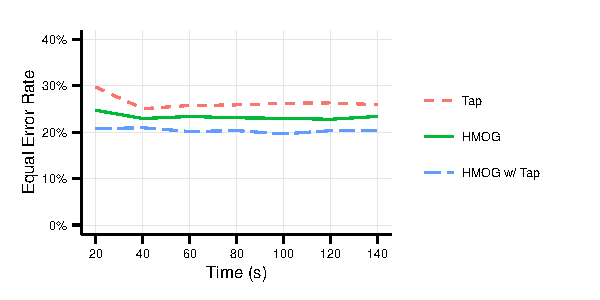
\includegraphics[width=1.1\linewidth]{plots_R/bkg_sitting}
\label{fig:bkg_sitting}}
\subfigure[EER for Walking]
{
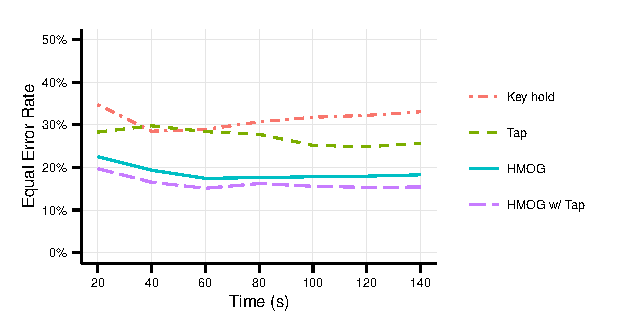
\includegraphics[width=1.1\linewidth]{plots_R/bkg_walking}
\label{fig:bkg_walking}}
\caption{EERs for BKG during sitting and walking. $X$-axis shows the authentication time in seconds.} %
\end{figure}
